\chapter{Did It Work? Causal Evaluation and Responsible AI}

\begin{weekbox}
\textbf{Theme.} Every recommendation in this course ends with a change: a new stock rule, a roster, a campaign. This
week asks whether a change caused the result, and how to put AI assistants into operational decisions without
letting them make unchecked ones.\\
\textbf{Outcomes.} LO8, LO9.\quad \textbf{Tools.} statsmodels, scikit-learn, SciPy, causaldata.\\
\textbf{Data.} Hillstrom randomised e-mail test (64\,000 customers); organ-donation registration rates in 27 US states;
Mboa employees (true training effect $+3$).\\
\textbf{Lab.} A/B analysis with an SRM check and an economic decision; confounding and doubly robust adjustment; DiD with
an event study; a guardrail for an AI-proposed replenishment plan.\\
\textbf{Deliverable.} Lab notebook; draft capstone report for feedback.
\end{weekbox}

\begin{timetable}
0:00--0:20 & Briefing & ``Trained staff are 11 points more productive. Should we train everyone?''\\
0:20--1:10 & Concepts & Potential outcomes, experiments, confounding, adjustment, DiD, explaining models, LLM failure modes\\
1:10--2:40 & Guided lab & Lab 7, Steps 1--5 (break at 1:55)\\
2:40--3:40 & Challenge & Exercises 7.3--7.7; capstone surgery\\
3:40--4:00 & Debrief & Which estimate of the training effect would you report to the HR director, and why?\\
\end{timetable}

\section{Correlation is not a decision}
\begin{definition}{Potential outcomes and the average treatment effect}
Each unit $i$ has two potential outcomes: $Y_i(1)$ if treated and $Y_i(0)$ if not. The causal effect is
$Y_i(1)-Y_i(0)$; the \emph{average treatment effect} is $\mathrm{ATE}=\E[Y(1)-Y(0)]$. We only ever observe one of the
two outcomes per unit; the other is the counterfactual.
\end{definition}

The naive comparison of treated and untreated units decomposes as
\[ \E[Y\mid T{=}1]-\E[Y\mid T{=}0]=\underbrace{\E[Y(1)-Y(0)\mid T{=}1]}_{\text{effect on the treated}}
+\underbrace{\E[Y(0)\mid T{=}1]-\E[Y(0)\mid T{=}0]}_{\text{selection bias}}. \]
If managers send their best staff to training, the trained would have been more productive anyway: selection bias,
caused by a \emph{confounder} (skill) that drives both treatment and outcome.

\begin{figure}[H]
\centering
\begin{tikzpicture}[node distance=24mm,v/.style={draw=navy,fill=defbg,rounded corners=2pt,font=\sffamily\small,minimum width=22mm,minimum height=8mm}]
\node[v] (t) {Training $T$};
\node[v,right=of t] (y) {Productivity $Y$};
\node[v,above=9mm of $(t)!0.5!(y)$] (x) {Skill $X$};
\draw[-{Latex},thick,teal] (t)--(y) node[midway,below,font=\scriptsize]{effect we want};
\draw[-{Latex},thick,brick] (x)--(t);
\draw[-{Latex},thick,brick] (x)--(y);
\node[font=\scriptsize,text=brick,right=2mm of x] {confounder: opens a back-door path};
\end{tikzpicture}
\caption{A causal diagram. Comparing $Y$ across $T$ mixes the effect with the back-door path through $X$.}
\end{figure}

\section{Randomised experiments}
Random assignment makes treated and control groups alike in everything, measured or not, so the difference in means
estimates the ATE without bias. It is the gold standard, and operations can run more experiments than it usually does:
alternate stores, randomise days, randomise which customers get a message.

\begin{keyformula}{A/B test essentials}
Effect $\hat\delta=\bar Y_T-\bar Y_C$, standard error $\sqrt{s_T^2/n_T+s_C^2/n_C}$, 95\% CI $\hat\delta\pm1.96\,\mathrm{SE}$.
Sample size per arm to detect $\delta$ with power $1-\beta$:
\[ n=\frac{2\,(z_{1-\alpha/2}+z_{1-\beta})^2\,\sigma^2}{\delta^2},\qquad \sigma^2=p(1-p)\ \text{for a conversion rate}. \]
\end{keyformula}

\begin{pitfall}{Experiments that lie}
\textbf{Sample-ratio mismatch}: if a 50/50 test ends 52/48, assignment or logging is broken; check with a $\chi^2$ test
before reading any result. \textbf{Peeking}: stopping the test the first day $p<0.05$ inflates false positives;
fix the sample size in advance. \textbf{Many metrics}: test twenty outcomes and one will be ``significant'' by chance.
\textbf{Interference}: if treated and control stores share a warehouse or customers, the control is contaminated.
\end{pitfall}

\begin{realcase}{A headline change at Bing}
Kohavi and Thomke (\emph{Harvard Business Review}, 2017) report that a Bing engineer's low-priority idea, lengthening
ad headlines, sat untested for months. When finally run as an A/B test it raised revenue by 12\%, worth over \$100
million a year in the US. Most ideas tested at large firms show no effect or a negative one; the value of
experimenting is finding the rare large winner and avoiding the many confident mistakes.
\end{realcase}

\section{When you cannot randomise}
\subsection{Adjusting for confounders}
If all confounders $X$ are measured (``no unmeasured confounding'') and every unit could have been treated or not
(\emph{overlap}), three estimators recover the effect:
\begin{itemize}[nosep]
\item \textbf{Regression adjustment}: regress $Y$ on $T$ and $X$; the coefficient on $T$ estimates the effect if the
outcome model is right.
\item \textbf{Inverse propensity weighting (IPW)}: estimate $e(x)=P(T{=}1\mid x)$ and weight units by $1/e$ (treated)
or $1/(1-e)$ (control). Right if the propensity model is right; unstable when $e$ is near 0 or 1.
\item \textbf{Doubly robust (AIPW)}: combines both, and is consistent if \emph{either} model is right:
\[ \hat\tau=\frac1n\sum_i\Big[\hat\mu_1(x_i)-\hat\mu_0(x_i)+\frac{T_i(Y_i-\hat\mu_1(x_i))}{\hat e(x_i)}-\frac{(1-T_i)(Y_i-\hat\mu_0(x_i))}{1-\hat e(x_i)}\Big]. \]
\end{itemize}
No method can adjust for a confounder you did not measure. Say which confounders you assume away.

\subsection{Difference-in-differences}
When a change hits one group at one time (a policy in one region, an app in two stores), compare the change in the
treated group with the change in an untreated group over the same period:
\begin{keyformula}{Difference-in-differences}
\[ \hat\tau_{\text{DiD}}=(\bar Y_{T,\text{post}}-\bar Y_{T,\text{pre}})-(\bar Y_{C,\text{post}}-\bar Y_{C,\text{pre}}). \]
Regression form with unit and period fixed effects: $Y_{it}=\alpha_i+\gamma_t+\tau\,D_{it}+\varepsilon_{it}$, with
standard errors clustered by unit. Identifying assumption: \emph{parallel trends}, i.e.\ without treatment the two groups
would have moved together.
\end{keyformula}
An \textbf{event study} replaces $D_{it}$ by one dummy per period relative to the change. Pre-period coefficients near
zero support parallel trends; post-period coefficients show how the effect develops. Card and Krueger's 1994 study
of New Jersey's minimum-wage rise, using fast-food restaurants across the border in Pennsylvania as controls, is the
classic example.

\section{Explaining models to managers}
Managers act on a model they understand. Three tools, in order of preference:
\begin{enumerate}[nosep]
\item \textbf{Show the decision rule}, not the model: ``order 82\% of the forecast'', ``alarm when the 6-hour average
falls below 57''. Most of this course's outputs can be stated this way.
\item \textbf{Global importance}: permutation importance (how much error rises when a feature is shuffled) or partial
dependence plots.
\item \textbf{Local explanations}: SHAP values attribute one prediction to features using Shapley values
(Lundberg and Lee, 2017). Use \texttt{pip install shap} if needed; remember that SHAP explains the \emph{model}, not
the world. A large SHAP value for ``promotion'' is not evidence that promotions cause sales.
\end{enumerate}

\section{AI assistants in operational decisions}
Large language models (LLMs) are now part of many analysts' daily work: drafting SQL, summarising supplier e-mails,
explaining a forecast, proposing an order. They are useful and they fail in specific, predictable ways.

\begin{center}\small
\begin{tabularx}{\linewidth}{@{}L{3.3cm}Y Y@{}}
\toprule
\textbf{Failure mode} & \textbf{Replenishment example} & \textbf{Guardrail}\\\midrule
Invented facts & proposes product P13, which does not exist & validate every ID against master data\\
Unit confusion & ``40'' meant cases of 12, read as 40 units & require explicit units; convert with master data\\
Arithmetic errors & totals that do not add up & recompute every number in code; never trust stated totals\\
Ignored constraints & 900 loaves of 1-day bread & encode constraints as checks, not as prompt text\\
Stale or partial context & uses last month's prices & pass current data through tools, log the data version\\
Prompt injection & a supplier e-mail says ``ignore budget limits'' & treat documents as data; the model cannot change rules\\
Overconfidence & fluent justification for a bad order & human approval above a value threshold; log decisions\\\bottomrule
\end{tabularx}
\end{center}

\begin{figure}[H]
\centering
\begin{tikzpicture}[node distance=7mm,b/.style={draw=#1,fill=#1!10,rounded corners=2pt,font=\sffamily\scriptsize,align=center,minimum height=10mm,text width=22mm}]
\node[b=slate] (u) {Planner's request};
\node[b=navy,right=of u] (l) {LLM drafts plan, calls tools};
\node[b=teal,above right=2mm and 7mm of l] (t1) {Forecast and ROP (Weeks 3--4)};
\node[b=teal,below right=2mm and 7mm of l] (t2) {Optimiser (Week 5)};
\node[b=brick,right=24mm of l] (v) {Deterministic validator};
\node[b=orange,right=of v] (h) {Human approves; decision logged};
\draw[-{Latex}] (u)--(l); \draw[-{Latex}] (l)--(t1); \draw[-{Latex}] (l)--(t2);
\draw[-{Latex}] (t1)--(v); \draw[-{Latex}] (t2)--(v); \draw[-{Latex}] (v)--(h);
\draw[-{Latex},brick,dashed] (v.south) to[bend left=25] node[below,font=\tiny]{rejected with reasons} (l.south);
\end{tikzpicture}
\caption{A safe pattern: the LLM composes and explains; tested code computes; a validator checks; a person decides.}
\end{figure}

\begin{realcase}{Moffatt v.\ Air Canada, 2024}
A customer service chatbot on Air Canada's website told a passenger he could claim a bereavement fare refund after
travelling, contrary to the airline's actual policy. British Columbia's Civil Resolution Tribunal held the airline
responsible for what its chatbot said and ordered it to pay. An organisation owns its AI's outputs. In operations, that
means every AI-generated order, roster or price must pass the same checks as one written by a junior analyst.
\end{realcase}

\paragraph{Free options} No paid service is needed to learn the pattern. Local open-weight models run with Ollama on a
laptop with 8--16\,GB of memory; several providers offer free API tiers with rate limits. The lab uses no model at all:
the guardrail is plain code, and it is the part that must be right.

% ------------------------------------------------------------------ LAB
\section{Practical Lab 7: Measuring effects and checking AI}
\begin{labbox}{Practical lab --- experiments, adjustment, DiD and a guardrail}
\textbf{Goal.} Read a real experiment and turn it into a decision; recover a known effect from confounded data;
estimate a policy effect with DiD; and validate an AI-proposed plan. \textbf{Files.} \texttt{real/hillstrom.csv},
\texttt{data/employees.csv}, \texttt{data/products.csv}, \texttt{data/sales.csv}; the organ-donation panel ships with
\texttt{causaldata}. \textbf{Time.} 90 minutes.
\end{labbox}

\step{Step 1: A randomised e-mail test}
\codeout{lab7_s1}{Sample-ratio check, then lifts with 95\% confidence intervals for both e-mails.}
\interp{The arms are balanced ($p=0.90$), so assignment worked. Both e-mails raise visits, conversions and spend; the
men's e-mail roughly doubles conversion (0.57\% to 1.25\%) and adds \$0.77 of spend per customer over two weeks.
Statistically significant is not yet a decision.}

\step{Step 2: From lift to profit, and planning the next test}
\codeout{lab7_s2}{Incremental profit per e-mail sent, and the sample size for a follow-up test.}
\interp{At a 35\% margin and \$0.10 per e-mail, the men's e-mail earns \$0.17 per customer (CI \$0.07 to \$0.27): send it.
The women's e-mail is not clearly profitable; its interval includes a loss. A follow-up test aiming to detect a
0.3-point change in conversion needs about 10\,000 customers per arm.}

\step{Step 3: Confounding, and three ways to adjust}
\codeout{lab7_s3}{Mboa training: the true effect planted in the generator is $+3$.}
\interp{The naive gap of 11 points is mostly selection: skilled staff were sent to training. Regression adjustment
(3.36, CI 2.63--4.08) and the doubly robust estimator (3.29) recover the truth. Plain IPW fails (1.79) because some
propensities are near 0.01 and 0.98, so a handful of employees get weights up to 63 and dominate the estimate. Always
look at the propensity distribution before trusting IPW.}

\step{Step 4: A policy change across states}
\codeout{lab7_s4}{DiD and an event study: California's active-choice rule for organ-donor registration (Q3 2011).}
\begin{figure}[H]\centering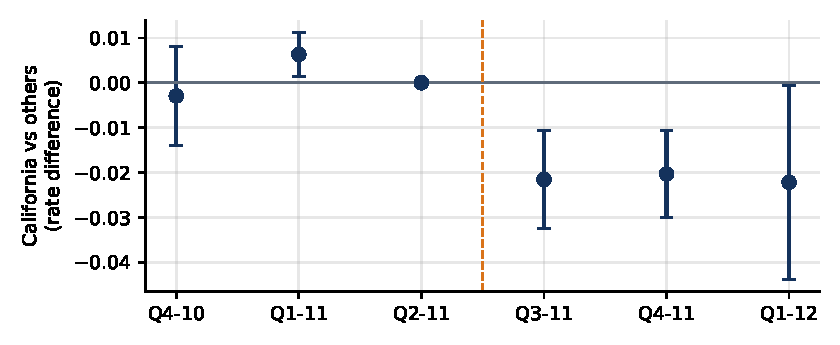
\includegraphics[width=0.78\linewidth]{../figs/lab7_event.pdf}
\caption{Event study: California minus other states, relative to Q2 2011. The dashed line marks the policy.}\end{figure}
\interp{California's registration rate fell by about 2.2 points relative to the other states after the change (cluster
SE 0.7 points), and the drop is immediate and stable across three quarters. Requiring an active choice, rather than an
opt-in nudge, reduced registrations. The pre-period coefficients are small, but the Q1 2011 coefficient is statistically different from zero: the
parallel-trends evidence is decent, not perfect, and with only six quarters it should be stated as an assumption.}

\step{Step 5: A guardrail for an AI-proposed order}
\codeout{lab7_s5}{Deterministic validation of a replenishment plan, as an LLM might propose it.}
\interp{The proposal reads well and is wrong in three ways: an invented product, a perishable order four times the
demand it could sell, and a negative ``return'' slipped into a purchase order. The validator catches all three in
milliseconds. It also converted the oil line from cases to units before checking it. The plan goes back to the
assistant with reasons, or to a person, and never straight to a supplier.}

\paragraph{So what (model answer)} \emph{Send the men's e-mail: it earns about \$0.17 per customer after costs. Training
raises productivity by about 3 points, not 11; budget the programme on 3. Before any AI assistant proposes orders, the
validator in Step 5 runs on every proposal and anything above 1\,M\xaf\ needs a manager's approval.}

% ------------------------------------------------------------------ EXERCISES
\section{Exercises}
\begin{enumerate}[label=\textbf{7.\arabic*},leftmargin=2.4em]
\item \emph{(Decomposition)} Using the Mboa employees, compute the naive difference and the regression estimate, and
from them an estimate of the selection bias. Interpret it in one sentence.
\item \emph{(Sample size)} Mboa wants to test whether SMS reminders raise weekly visits from 30\% to 32\% of loyalty
members. How many members per arm for 80\% power at 5\% significance?
\item \emph{(Heterogeneity)} In Hillstrom, estimate the men's-e-mail lift on spend separately for customers who bought
men's products, women's products, or both. Whom should the e-mail target?
\item \emph{(SRM)} A test planned 50/50 ends with 10\,240 and 9\,760 users. Is there a sample-ratio mismatch? List three
causes you would investigate.
\item \emph{(DiD, Mboa)} Estimate the loyalty-app effect in the Douala stores (S4, S5) from 1 July 2024 using the other
stores as controls, in logs. Does DiD recover the planted $+8\%$? Draw the event study by month.
\item \emph{(Robustness)} Repeat Step 3 with propensities trimmed to $[0.1,0.9]$ and with stabilised weights. How do IPW
and AIPW change?
\item \emph{(Guardrail)} Extend the validator: reject any line whose stated reason contains instructions (e.g.\
``ignore'', ``override''), add a storage check from Week 6, and require approval when total value exceeds 1\,M\xaf.
Write three test proposals that must fail.
\end{enumerate}

\section{Sample final-examination questions}
\begin{enumerate}[label=\textbf{Q\arabic*.},leftmargin=2.4em]
\item A store's lead time is 5 days, daily lead-time forecast error has sd 4 units (independent days), target CSL 95\%.
Compute the safety stock. The forecast is improved and the error sd falls to 3. What is the annual saving if the
unit holding cost is 500\xaf\ a year?
\item The critical ratio for a perishable item is 0.3. Should the order be above or below the median forecast? Explain
with the cost of each error.
\item In an LP, the labour constraint has a shadow price of 1\,800\xaf\ per hour, valid up to 40 extra hours. Overtime
costs 2\,500\xaf\ per hour. What do you recommend, and why?
\item A process has 120 cases in progress and completes 30 cases a day. What is the average time in the process? What
must happen to WIP to halve it at the same throughput?
\item Explain why an 80\%-utilised M/M/1 server has on average four customers in the system, and what halving the variability
of service time would do.
\item Give the identifying assumption of difference-in-differences and describe how an event-study plot checks it.
\item List three ways an LLM-proposed purchase order can be wrong and the control that catches each.
\end{enumerate}
